\chapter{Pattern matching}
\section{Algoritmi di string matching esatto}

\subsection*{Automa a stati finiti}
Un generico automa a stati finiti è una quintupla:
\begin{center}
    $(Q, \Sigma, \delta, q_0, F)$
\end{center}
dove:
\begin{itemize}
    \item $Q$ è un insieme finito di stati;
    \item $\Sigma$ è un insieme finito di simboli di input;
    \item $\delta$ è la funzione di transizione. È definita come $\delta: Q \times \Sigma \rightarrow Q$;
    \item $q_0$ è lo stato iniziale. $q_0 \in Q$;
    \item $F$ è un insieme finito di stati finali. Vale $F \subseteq Q$.
\end{itemize}
Gli automi a stati finiti possono riconoscere solo i linguaggi regolari, ovvero quelli generati da grammatiche di tipo 3 (grammatiche lineari sinistre o destre).\\
Ogni pattern genera un automa differente e riconosce, quindi, un linguaggio differente.
Dato un pattern $P$, l'automa a stati finiti che lo riconosce è definito come:
\begin{itemize}
    \item $Q = \left\{ 0, 1, \ldots, m \right\}$;
    \item $\Sigma = $ insieme dei simboli su cui sono definiti pattern e testo; 
    \item $\delta : \{ 0, \ldots, m \} \times \Sigma \rightarrow \{ 0, \ldots, m \}$;
    \item $q_0 = 0$;
    \item $F = \{ m \}$
\end{itemize}


\subsubsection{Preprocessing del pattern: costruzione della funzione di transizione}
Durante la fase di preprocessing, l'algoritmo calcola la funzione di transizione.
È però prima necessario introdurre la nozione di \textit{bordo di una stringa}. Sia $W = \langle w_1, \ldots, w_m \rangle$ una stringa, il bordo $B(W)$ è il suo più lungo prefisso proprio che è anche suo suffisso, ovvero una sottostringa $B = \langle b_1, \ldots, b_k \rangle$, $k < m$, tale che:
\begin{center}
    $b_1 = w_1 \land \ldots \land b_k = w_k \quad \textnormal{e} \quad b_1 = w_{n-k+1} \land \ldots \land b_k = w_n$
\end{center} 
Dato un pattern $P$ e detti $j$ lo stato corrente dell'automa, per cui $P[1:j]$ è match esatto, e $\sigma$ il simbolo ricevuto in input dall'automa, allora la funzione di transizione è definita come:
\begin{center}
    $\delta (j, \sigma) = \begin{cases}
        j+1 & \quad j < m \land P[j+1] = \sigma \\
        \vert \textnormal{B}(P[1:j]\sigma) \vert & \quad j = m \lor P[j+1] \neq \sigma 
    \end{cases}$
\end{center}
La funzione di transizione viene memorizzata in una tabella $|P| \times |\Sigma|$, dove le righe rappresentano lo stato corrente, mentre le colonne il simbolo ricevuto in input.
La cella di indici $(i, j)$ conterrà quindi $\delta (i, \sigma_j)$, dove $\sigma_j$ è il simbolo associato all'indice $j$.

Esiste un algoritmo per il riempimento della tabella, di complessità $O(|P| \times |\Sigma|)$, che calcola induttivamente i valori della riga di indice $i$ a partire da quelli contenuti nella riga $i-1$ (non visto a lezione). 

\subsubsection{Scansione del testo}
La scansione del testo è molto semplice, e viene effettuata utilizzando la tabella definita nella fase di preprocessing.

Detto $i$ lo stato corrente dell'automa, e $\sigma$ il simbolo ricevuto in input, allora l'automa passerà nello stato $\delta (i, \sigma)$, contenuto nella cella di indici $(i, j)$ della tabella, con $j$ tale che $\sigma_j = \sigma$.
Ogni qualvolta l'automa entra nello stato accettante $m$, l'algoritmo ha rilevato un'occorrenza esatta e, quindi, ritorna la sua posizione di inizio $i - |P| + 1$.

La valutazione del testo T, e quindi la computazione dell'automa, genera una sequenza di stati attraversati di lunghezza $|T|$.

\begin{thm}
    Sia $\langle j_0, \ldots, j_{|T|} \rangle$ la sequenza di stati attraversati nella scansione, allora $j_i$ indica la lunghezza del più lungo prefisso di $P$ che è suffisso di $T[1:i]$.
\end{thm}
Dovendo modificare lo stato dell'automa per ogni singolo simbolo letto dal testo, la complessità temporale della scansione con automa a stati finiti è $\Theta(n)$.



\subsection*{Algoritmo di Knuth-Morris-Pratt}
L'algoritmo di Knuth-Morris-Pratt (KMP) è un algoritmo di string matching esatto, detto anche automa compatto, in quanto costruisce un automa indipendente dalla dimensione dell'alfabeto.

Di base, KMG si comporta come l'automa a stati finiti, ma implementa alcune tecniche che permettono uno spostamento più efficiente della finestra e di evitare di ricontrollare il pattern dalla prima posizione a ogni spostamento della finestra.

\subsubsection{Preprocessing del pattern: calcolo della prefix function}
Durante la fase di preprocessing, l'algoritmo analizza il pattern e calcola la \textit{prefix function} (detta anche funzione di fallimento) $\varphi$, una funzione che permetterà di calcolare efficientemente, in caso di fallimento, la nuova posizione di inizio della finestra e la posizione del pattern da cui riprendere il confronto.

In particolare, la prefix function specifica, per ogni posizione $j$ del pattern, come l'algoritmo deve comportarsi quando $P[j]$ è il simbolo del pattern a causare il mismatch, supponendo che $P[1:j-1]$ non abbia generato fallimenti di match per la finestra corrente.
Se $P[j]$ è il simbolo che porta al fallimento, allora $j$ viene detta \textit{posizione di mismatch}.

Per ogni posizione del pattern $j$ (rappresentante il prefisso $P[1:j]$), compreso il valore 0 (rappresentante la stringa vuota $\epsilon$), la prefix function viene calcolata come:
\begin{center}
    $\varphi(j) = \begin{cases}
        -1 & j = 0 \\
        |\textnormal{B}(P[1:j])| & j > 0
    \end{cases}$
\end{center}
Dovendo calcolare e memorizzare un valore per ogni posizione del pattern e per la posizione fittizia di indice 0, allora:
\begin{center}
    Complessità temporale: $O(|P|)$\\
    Complessità spaziale: $O(|P|)$
\end{center}
Di conseguenza, il calcolo della prefix function è più efficiente del calcolo della funzione di transizione dell'automa a stati finiti, che richiede, invece, tempo $O(|\Sigma| \cdot |P|)$.
\subsubsection{Scansione del testo}
La scansione del testo, una volta calcola la prefix function, è molto semplice da effettuare.

Siano $i$ la posizione di inizio della finestra corrente, $j$ la posizione all'interno del pattern corrente, e $P[1:j-1]$ il prefisso del pattern per cui si ha match esatto con i primi $j-1$ caratteri della finestra corrente.
\begin{itemize}
    \item Se $T[i + j - 1] = P[j]$, allora incrementa $j$ e prosegui con il    confronto per la finestra corrente.\\
    \item Se $T[i + j - 1] \neq P[j]$, allora sposta la finestra in modo che la nuova posizione di inizio sia:
    \begin{center}
        $i + j - \varphi(j-1) - 1$
    \end{center}
    Ma, per definizione di bordo, i primi $\varphi(j - 1)$ caratteri della nuova finestra sono già in match esatto con il pattern.
    Di conseguenza, il confronto ricomincierà da:
    \begin{center}
        $\textnormal{Pattern: } \begin{cases}
            1 & \quad j = 1 \\
            \varphi(j-1) + 1 & \quad j > 1
        \end{cases}$
    \end{center}
    \begin{center}
        $\textnormal{Testo: } \begin{cases}
            i + 1 & \quad j = 1 \\
            i + j - 1 & \quad j > 1
        \end{cases}$
    \end{center}
\end{itemize}
L'algoritmo rileva un'occorrenza esatta sse riesce a effettuare un match esatto tra la finestra corrente e il pattern: in questo caso, viene restituita la posizione $i$, ovvero l'inizio dell'occorrenza esatta.

La scansione ha complessità lineare $\Theta(n)$. Le costanti di crescita sono però maggiori rispetto a quelle della scansione tramite automa a stati finiti: di conseguenza, la scansione di KMP è più lenta rispetto a quella dell'automa.

%\begin{algorithm}[H]
%    \caption{Algoritmo KMP per la ricerca delle occorrenze esatte.}
%    \label{alg:kmp}
%    \begin{algorithmic}[1]
%        \Procedure{KMP-search}{P, T, $\varphi$}
%            \State m $\gets$ $\vert$P$\vert$
%            \State n $\gets$ $\vert$T$\vert$
%            \State j $\gets$ 0
%            \For{q $\gets$ 1 to n}
%                \While{j $\ge$ 0 $\land$ P[j+1] $\neq$ T[q]}
%                    \State j $\gets$ \Call{$\varphi$}{j}
%                \EndWhile
%                \State j $\gets$ j+1
%                \If{j = m}
%                    \State \Return q - m + 1
%                \EndIf
%            \EndFor
%        \EndProcedure
%    \end{algorithmic}
%\end{algorithm}


\subsection*{Algoritmo di Baeza-Yates e Gonnet}
L'algoritmo di Baeza-Yates e Gonnet (BYG) è un algoritmo di string matching esatto basato sul paradigma Shift-And.
Esso può essere applicato sse la lunghezza del pattern è minore o uguale alla lunghezza della word del calcolatore che lo implementa, in quanto devono essere eseguite operazioni bit a bit su parole di lunghezza pari a quella del pattern.

\subsubsection{Word di bit e operazioni bit a bit}
Per poter capire l'algoritmo, è necessario introdurre il concetto di word di bit: una word è un gruppo di bit trattato come un'unità, rappresentante un valore di un certo tipo.
Le operazioni su word hanno complessità costante $O(1)$ e sfruttano il $bit-parallelism$: il processore, infatti, applica la stessa operazione a tutti i bit della word contemporaneamente, non sequenzialmente.\\
D'ora in poi, l'indicizzazione delle posizioni di una word partirà da sinistra e inizierà da 1.

Le principali operazioni bit a bit su word sono:
\begin{itemize}
    \item AND: date due stringhe binarie $w_1$ e $w_2$, entrambe di lunghezza $n$, l'operazione ritorna una nuova stringa binaria $w$ di lunghezza $n$ tale che:
    \begin{center}
        $w[i] = w_1[i] \textnormal{ AND } w_2[i]$
    \end{center}
    \item OR: date due stringhe binarie $w_1$ e $w_2$, entrambe di lunghezza $n$, l'operazione ritorna una nuova stringa binaria $w$ di lunghezza $n$ tale che:
    \begin{center}
        $w[i] = w_1[i] \textnormal{ OR } w_2[i]$
    \end{center}
    \item RSHIFT: shift, di una posizione a destra, di tutti i bit, rendendo il bit più significativo uguale a 0.
    Data una stringa binaria $w_1$ di lunghezza $n$, restituisce una nuova stringa binaria $w$ di lunghezza $n$ tale che:
    \begin{equation*}
        w[i] = \begin{cases}
            0 & i = 1 \\
            w_1[j-1] & i > 1
        \end{cases}
    \end{equation*}
    \item RSHIFT1: shift, di una posizione a destra, di tutti i bit, rendendo il bit più significativo uguale a 1.
    Data una stringa binaria $w_1$ di lunghezza $n$, restituisce una nuova stringa binaria $w$ di lunghezza $n$ tale che:
    \begin{equation*}
        w[i] = \begin{cases}
            1 & i = 1 \\
            w_1[j-1] & i > 1
        \end{cases}
    \end{equation*}
    Non esiste un operatore di RSHIFT1. Questa operazione viene quindi implementata usando RSHIFT e OR:
    si esegue prima l'operazione di RSHIFT su $w_1$, e poi il risultato viene posto in OR con la maschera $10\ldots00$.
    Per generare questa maschera, definisco la stringa $00\ldots01$ ed eseguo $|P|- 1$ operazioni di LSHIFT su essa.
\end{itemize}

\subsubsection{Preprocessing del pattern: calcolo delle parole di occorrenza}
La prima fase eseguita dal Baeza-Yates è quella di preprocessing, in cui viene analizzato il pattern e vengono generate le \textit{parole di occorrenza}.
Sia $\Sigma$ l'alfabeto dei possibili simboli, allora dovranno essere calcolate $|\Sigma|$ parole di occorrenza, ognuna associata a un certo simbolo e di lunghezza pari a $|P|$, con $P$ pattern.
Di conseguenza, la memoria richiesta per memorizzare tutte le parole è pari a $O(|\Sigma| \cdot |P|)$.

Una parola di occorrenza $B_{\sigma}$, definita sul simbolo $\sigma$, indica tutte le posizioni del pattern in cui compare $\sigma$:
\begin{center}
    $B_{\sigma}[i] = 1 \longleftrightarrow P[i] = \sigma$
\end{center}
L'algoritmo con cui calcolare le parole di occorrenza è il seguente:
\begin{enumerate}
    \item tutte le $|\Sigma|$ parole di lunghezza $|P|$ vengono inizializzate a $0\ldots0$;
    \item viene creata una maschera $M$ con il solo bit più significativo uguale a 1, a partire dalla stringa $0\ldots01$ ed effettuando $|P| - 1$ operazioni di LSHIFT;
    \item viene scandito il pattern.
    Sia $i$ la posizione corrente sul pattern, e $B_{P[i]}$ la parola di occorrenza associata al simbolo $P[i]$, allora verrà effettuata l'operazione:
    \begin{center}
        $B_{P[i]} = M \textnormal{ OR } B_{P[i]}$\\
        $M = \textnormal{RSHIFT}(M)$
    \end{center}
    L'operazione di RSHIFT sulla maschera serve a scorrere l'unico bit impostato a 1 al suo interno: infatti, essendo $|M| = |P|$, esso corrisponde alla posizione corrente all'interno del pattern, e deve quindi scorrere mano a mano che la scansione del pattern procede.
\end{enumerate}
La fase di preprocessing ha complessità:
\begin{center}
    $O(|\Sigma| + |P|)$
\end{center}
$O(|\Sigma|)$ deriva dall'inizializzazione delle $|\Sigma|$ parole (l'inizializzazione di una singola parola è costante), mentre $O(|P|)$ è il tempo richiesto per valutare tutte le celle del pattern.

\subsubsection{Scansione del testo}
La scansione del testo non prevede confronti espliciti tra simboli del testo e simboli del pattern, ma è basata su \textit{confronti impliciti}.

Per ogni posizione $i$ del testo, viene calcolata la parola $D_i$, di lunghezza $|P|$, che contiene informazioni riguardo 
il match tra prefissi del pattern e suffissi di $T[1:i]$:
\begin{center}
    $D_i[j] = 1 \longleftrightarrow P[1:j] == \textnormal{suff}(T[1:i])$
\end{center}
Di conseguenza, fissata una posizione $i$ nel testo, la parola $D_i$ specifica quali prefissi del pattern sono suffissi di $T[1:i]$.

L'algoritmo rileva un'occorrenza esatta sse $D_i[|P|] = 1$, ovvero il bit meno significativo di $D_i$ è 1, e la posizione di inizio dell'occorrenza sarà:
\begin{center}
    $i-m+1$
\end{center}
Il calcolo di $D_i$ viene effettuato anche per $i=0$, nonostante $D_0[j] = 0, \; \forall j, 1 \le j \le |P|$: sarà infatti il caso base da cui si inizierà a calcolare tutte le successive $D_i.$

Queste parole non vengono in realtà tutte calcolate e memorizzate: $D_i$ viene definita induttivamente utilizzando $D_{i-1}$, e $D_0$ funge da caso base da cui parte il calcolo delle parole. Di conseguenza, sarà necessario in un certo istante dell'esecuzione dell'algoritmo solo una parole $D_i$, e sarà quindi richiesta solo una memoria pari a $|P|$.

Un algoritmo generico per la scansione del testo è quindi:
\begin{enumerate}
    \item inizializza $D_0$;
    \item se $D_i[|P|] = 1$, ovvero il bit meno significativo d $D_i$ è pari a 1, allora si è rilevata un'occorrenza esatta. Viene quindi restituito l'indice $i-m+1$, corrispondente alla posizione di inizio dell'occorrenza esatta;
    \item calcola $D_{i+1}$;
    \item torna al punto 2
\end{enumerate}

È stato detto che l'algoritmo calcola $D_{i+1}$ induttivamente, a partire da $D_i$. In particolare, è stato detto che:
\begin{center}
    $D_i[j] = 1 \longleftrightarrow P[1:j] == \textnormal{suff}(T[1:i])$
\end{center} 
Ma si può affermare che:
\begin{center}
    $P[1:j] == \textnormal{suff}(T[1:i]) \longleftrightarrow P[1:j-1] == \textnormal{suff}(T[1:i-1]) \textnormal{ AND } T[i] == P[j]$
\end{center}
e $D_i[j]$ potrà quindi essere calcolato come:
\begin{center}
    $D_i[j] = P[1:j-1] == \textnormal{suff}(T[1:i-1]) \textnormal{ AND } T[i] == P[j]$
\end{center}
Si è quindi definito il calcolo di $D_i$ ricorsivamente, utilizzando informazioni relative a $D_{i-1}$. Si può affermare che $P[1:j-1] == \textnormal{suff}(T[1:i-1])$ è vero solo se $D_{i-1}[j-1] = 1$.
Per quanto riguarda la seconda parte, ovvero $T[i] == P[j]$, essa è vera sse $B_{T[i]}[j] = 1$.

Di conseguenza, se $j > 1$, si può calcolare $D_i[j]$ come:
\begin{center}
    $D_i[j] = D_{i-1}[j-1] \textnormal{ AND } B_{T[i]}[j] \quad \quad \textnormal{sse } j > 1$
\end{center}
Per $j = 1$ è necessario definire un caso particolare, in quanto l'utilizzo della regola precedente porterebbe altrimenti a $D_{i-1}[0]$, che per l'indicizzazione dei bit adottata non avrebbe alcun senso.
Si ritorna quindi alla definizione originale non ricorsiva, ovvero $D_i[j] = 1 \longleftrightarrow P[1:j] == \textnormal{suff}(T[1:i])$.

Essendo $j = 1$, allora:
\begin{center}
    $P[1:j] = P[1:1] = P[1]$
\end{center}
Inoltre $\textnormal{suff}(T[1:i])$ deve essere di lunghezza 1, quindi:
\begin{center}
    $\textnormal{suff}(T[1:i]) = T[i]$
\end{center} 
La regola non ricorsiva può quindi essere riscritta come:
\begin{center}
    $D_i[j] = P[j] == T[i] \rightarrow D_i[j] = B_{T[i]}[j] \quad \quad \textnormal{sse } j = 1$
\end{center}
che a sua volta può essere scritta, senza modificare il suo significato, come:
\begin{center}
    $D_i[j] = 1 \textnormal{ AND } B_{T[i]}[j] \quad \quad \textnormal{sse } j = 1$
\end{center}
Si ha quindi:
\begin{center}
    $D_i[j] = \begin{cases}
        D_{i-1}[j-1] \textnormal{ AND } B_{T[i]}[j] & j > 1 \\
        1 \textnormal{ AND } B_{T[i]}[j] & j = 1
    \end{cases}$
\end{center}
Ma, effettuando l'operazione di RSHIFT1 di $D_{i-1}$, allora $D_{i-1}[j-1] = D_{i-1}[j]$ e $D_{i-1}[j]$ DA FARE . Sostituendo nelle formule fino ad ora trovate si ottiene:
\begin{center}
    $D_i[j] = \begin{cases}
        \textnormal{RSHIFT1}(D_{i-1})[j] \textnormal{ AND } B_{T[i]}[j] & j > 1 \\
        \textnormal{RSHIFT1}(D_{i-1})[j] \textnormal{ AND } B_{T[i]}[j] & j = 1
    \end{cases}$\\
    \big\downarrow\\
    $D_i[j] = \textnormal{RSHIFT1}(D_{i-1})[j] \textnormal{ AND } B_{T[i]}[j]$
\end{center}
Utilizzando questa formula, però, ogni bit della parola $D_i$ viene aggiornato $|T|$ volte indipendentemente dagli altri. Di conseguenza, la complessità è $O(|P| \cdot |T|)$.
È possibile, però, sfruttare il bit-parallelism del processore, in modo che tutti i bit della parola $D_i$ vengano aggiornati contemporaneamente, e la complessità si riduce così a $\Theta(|T|)$.
Per farlo, la formula viene ridefinita come:
\begin{center}
    $D_i = \textnormal{RSHIFT1}(D_{i-1}) \textnormal{ AND } B_{T[i]}$
\end{center}

\subsection*{Confronto tra algoritmi di string matching esatto}
\begin{table}[h]
    \centering
    \begin{tabular}{|c|c|c|c|}
    \hline
                                                                  & Automa                       & KMP           & BYG                          \\ \hline
    Memoria                                                       & $\Theta(|P| \cdot |\Sigma|)$ & $\Theta(|P|)$ & $\Theta(|\Sigma| \cdot |P|)$ \\ \hline
    \begin{tabular}[c]{@{}c@{}}Tempo\\ Preprocessing\end{tabular} & $\Theta(|\Sigma| \cdot |P|)$ & $\Theta(|P|)$ & $\Theta(|\Sigma| + |P|)$     \\ \hline
    \begin{tabular}[c]{@{}c@{}}Tempo\\ Scansione\end{tabular}     & $\Theta(n)$                  & $O(n)$        & $O(n)$                       \\ \hline
    \end{tabular}
    \caption{Complessità degli algoritmi di string matching esatto.}
    \label{tab:exact_string_match}
\end{table}
Si può notare che tutti gli algoritmi presentano una complessità di scansione lineare in $n$. 
Essi però, nella pratica, si differenziano molto. L'algoritmo più performante è, infatti, BYG, che però presenta come grosso svantaggio quello di essere applicabile solo su pattern di lunghezza inferiore alla word del calcolatore che implementa l'algoritmo. Per quanto riguarda KMP e l'automa a stati finiti, invece, le costanti di crescita nascoste della complessità di scansione non sono affatto uguali: KMP è infatti meno performante nella scansione rispetto all'automa. KMP presenta però come vantaggio un utilizzo minore di memoria e una fase di preprocessing molto rapida, soprattutto se paragonata a quella dell'automa. 

Ciascun algoritmo è quindi consigliato nelle seguenti situazioni:
\begin{itemize}
    \item singolo pattern di dimensione minore della dimensione della word e singolo testo $\longrightarrow$ BYG;
    \item singolo pattern di dimensione maggiore della dimensione della word e singolo testo $\longrightarrow$ KMP;
    \item tanti pattern su un singolo testo $\longrightarrow$ KMP.\\
    Essendo presenti molti pattern, si vuole evitare di utilizzare troppa memoria per gestirli. Di conseguenza, KMP permette di risparmiare memoria rispetto all'automa, oltre che avere una fase di preprocessing più rapida. La scansione richiederà più tempo, ma dovendo effettuarla, per ogni pattern, una sola volta (in quanto si ha un solo testo), allora va bene.
    \item singolo pattern su tanti testi $\longrightarrow$ automa a stati finiti.\\
    L'automa ha, dopo una fase di preprocessing più onerosa rispetto a KMP, una scansione molto rapida: siccome la scansione deve essere ripetuta più volte su diversi testi, allora è vantaggioso avere una scansione più rapida. Si sacrificherà più memoria, in confronto all'utilizzo di KMP, ma essendo un solo pattern non se ne occupa molta;
    \item tanti pattern su tanti testi $\longrightarrow$
\end{itemize}

\section{Algoritmi di string matching approssimato}
\subsection*{Algoritmo di Wu e Manber}
L'algoritmo di Wu e Manber si può considerare un'estensione dell'algoritmo di Baeza-Yates: anch'esso, infatti, adotta il bit-parallelism ed è basato sul paradigma shift-and.
WM riceve in input un testo $T, |T| = n$, un pattern $P, |P|=m$ e una soglia di errore $k$, e restituisce tutte le posizioni $i$ del testo che sono fine di un'occorrenza approssimata.

\subsubsection{Preprocessing del pattern: calcolo delle parole di occorrenza}
La prima fase eseguita dal Wu-Manber è quella di preprocessing, in cui viene analizzato il pattern e vengono generate le parole di occorrenza. Sia $\Sigma$ l'alfabeto dei possibili simboli, allora dovranno essere calcolate $|\Sigma|$ parole di occorrenza, ognuna associata a un certo simbolo e di lunghezza pari a $|P|$.
Di conseguenza, la memoria richiesta per memorizzare tutte le parole è pari a $O(|\Sigma| \cdot |P|)$.

Una parola di occorrenza $B_{\sigma}$, definita sul simbolo $\sigma$, indica tutte le posizioni del pattern in cui compare $\sigma$:
\begin{center}
    $B_{\sigma}[i] = 1 \longleftrightarrow P[i] = \sigma$
\end{center}
L'algoritmo con cui calcolare le parole di occorrenza è il seguente:
\begin{enumerate}
    \item tutte le $|\Sigma|$ parole di lunghezza $|P|$ vengono inizializzate a $0\ldots0$;
    \item viene creata una maschera $M$ con il solo bit più significativo uguale a 1, a partire dalla stringa $0\ldots01$ ed effettuando $|P| - 1$ operazioni di LSHIFT;
    \item viene scandito il pattern.
    Sia $i$ la posizione corrente sul pattern, e $B_{P[i]}$ la parola di occorrenza associata al simbolo $P[i]$, allora verrà effettuata l'operazione:
    \begin{center}
        $B_{P[i]} = M \textnormal{ OR } B_{P[i]}$\\
        $M = \textnormal{RSHIFT}(M)$
    \end{center}
    L'operazione di RSHIFT sulla maschera serve a scorrere l'unico bit impostato a 1 al suo interno: infatti, essendo $|M| = |P|$, esso corrisponde alla posizione corrente all'interno del pattern, e deve quindi scorrere mano a mano che la scansione del pattern procede.
\end{enumerate}
La fase di preprocessing ha complessità:
\begin{center}
    $O(|\Sigma| + |P|)$
\end{center}
$O(|\Sigma|)$ deriva dall'inizializzazione delle $|\Sigma|$ parole (l'inizializzazione di una singola parola è costante), mentre $O(|P|)$ è il tempo richiesto per valutare tutte le celle del pattern.

\subsubsection{Scansione del testo}
La scansione del testo non prevede confronti espliciti tra simboli del testo e simboli del pattern, ma è basata su confronti impliciti.

Viene innanzitutto introdotto un nuovo indice $h, 0 \le h \le k$, che indica il numero di errori per una certa occorrenza.
$P[1:j] = \textnormal{suff}_h(T[1:i])$ indica, invece, che il prefisso di lunghezza $j$ del pattern è suffisso di $T[1:i]$ a meno di massimo $h$ errori.

Le parole calcolate sul testo $D_i^h$ dipendono ora da due parametri: la posizione corrente nel testo $i$ e il numero massimo di errori $h$.

$D_i^h[j] = 1$ sse il prefisso di lunghezza $j$ del pattern è suffisso di $T[1:i]$ a meno di massimo $h$ errori.
Come per l'algoritmo di Baeza-Yates, se $D_i^h[m] = 1$, ovvero il bit meno significativo di $D_i^h$ è 1, $i$ è la posizione di fine di un'occorrenza approssimata del pattern, a meno di massimo $h$ errori. Essendo, però, l'algoritmo applicato su una soglia di errore $k$, allora l'occorrenza approssimata viene restituita solo quanto $h = k$.

$D_i^0, 0 \le i \le |T|$, ovvero le parole che ammettono al massimo 0 errori, equivalgono alle parole calcolate nel corso dell'esecuzione dell'algoritmo di Baeza-Yates.

$D_0^h, 0 \le h \le k$, ovvero le parole sul prefisso vuoto del testo e che ammettono un qualsiasi numero di errori, avranno solo i primi $h$ impostati a 1, mentre il resto della parola sarà composto da soli bit impostati a 0. 
\begin{center}
    $D_0^h[j] = \begin{cases}
        1 & j \le h \\
        0 & j > h
    \end{cases}$
\end{center}
Si hanno quindi i casi base per $h = 0$ e $i = 0$.
Per calcolare la generica $D_i^h, i > 0 \land h > 0$, invece, $D_i^h[j] = 1$ sse si verifica uno dei seguenti casi:
\begin{itemize}
    \item $P[1:j-1] = \textnormal{suff}_h(T[1:i-1]) \textnormal{ AND } P[j] = T[i]$
    \item $P[1:j-1] = \textnormal{suff}_{h-1}(T[1:i-1])$\\
        $\Updownarrow$ \\
        sostituzione di $T[i]$ con $P[j]$ o sostituzione di $P[j]$ con $T[i]$;
    \item $P[1:j-1] = \textnormal{suff}_{h-1}(T[1:i])$ \\
    $\Updownarrow$ \\
    inserimento di $P[j]$ come ultimo elemento del testo;
    \item $P[1:j] = \textnormal{suff}_{h-1}(T[1:i-1])$ \\
    $\Updownarrow$ \\
    inserimento di $T[i]$ come ultimo elemento del pattern.
\end{itemize}
Tramite manipolazione simbolica dei precedenti casi:
\begin{itemize}
    \item $P[1:j-1] = \textnormal{suff}_h(T[1:i-1]) \textnormal{ AND } P[j] = T[i]$ \\
    $\Updownarrow$ \\
    $D_{i-1}^h[j-1] \textnormal{ AND } P[j] = T[i]$
    \item $P[1:j-1] = \textnormal{suff}_{h-1}(T[1:i-1])$\\
    $\Updownarrow$ \\
    $D_{i-1}^{h-1}[j-1]$
    \item $P[1:j-1] = \textnormal{suff}_{h-1}(T[1:i])$\\
    $\Updownarrow$\\
    $D_i^{h-1}[j-1]$
    \item $P[1:j] = \textnormal{suff}_{h-1}(T[1:i-1])$\\
    $\Updownarrow$\\
    $D_{i-1}^{h-1}[j]$
\end{itemize}
Si hanno ancora comunque casi separati per $j = 1$ e $j > 1$.
Per poter unificarli, è necessario trovare un modo di rimuovere $j-1$ dal caso $j>1$, perchè per $j = 1$ ciò genererebbe 0, che è ovviamente un indice non valido per il pattern.
Ma:
\begin{center}
    $D_{i-1}^h[j-1] = \textnormal{RSHIFT1}(D_{i-1}^h)[j]$\\
    $D_{i-1}^{h-1}[j-1] = \textnormal{RSHIFT1}(D_{i-1}^{h-1})[j]$\\
    $D_i^{j-1}[j-1] = \textnormal{RSHIFT1}(D_i^{h-1}[j])$
\end{center}
Di conseguenza:
\begin{center}
    $D_i^h[j] = (\textnormal{RSHIFT1}(D_{i-1}^h)[j] \textnormal{ AND } P[j] = T[i])$\\
    $\textnormal{OR } \textnormal{RSHIFT1}(D_{i-1}^{h-1})[j]$\\
    $\textnormal{OR } \textnormal{RSHIFT1}(D_i^{h-1})[j]$\\
    $\textnormal{OR } D_{i-1}^{h-1}[j]$\\
    $\forall j, 1 \le j \le |P|$
\end{center}
L'algoritmo generico per la scansione del testo in Wu e Manber è:
%\begin{algorithm}[H]
%    \caption{Scansione del testo nell'algoritmo Wu e Manber}
%    \label{alg:wu_manber_search}
%    \begin{algorithmic}[1]
%        \State $D_0^0$ $\gets$ $\underbrace{0\ldots0}_{|P|}$
%        \For{i $\gets$ 1 to $|T|$}
%            \State $D_i^0$ $\gets$ $\textnormal{RSHIFT1}(D_{i-1}^0) \textnormal{ AND } B_{T[i]}$
%        \EndFor
%        \For{h $\gets$ 1 to k}
%            \State $D_0^h$ $\gets$ $\underbrace{1\ldots1}_h \underbrace{0\ldots0}_{|P| - h}$
%            \For{i $\gets$ 1 to $|T|$}
%                \State $D_i^h$ $\gets$ $(\textnormal{RSHIFT1}(D_{i-1}^h) \textnormal{ AND } P[j] = T[i]) \textnormal{ OR }
%                \textnormal{RSHIFT1}(D_{i-1}^{h-1}) \textnormal{ OR }$ \\$
%                \textnormal{RSHIFT1}(D_i^{h-1}) \textnormal{ OR } 
%                D_{i-1}^{h-1}$
%                \If{h = k AND $D_i^h[|P|]$ = 1}
%                    \State \Return i
%                \EndIf
%            \EndFor
%        \EndFor
%    \end{algorithmic}
%\end{algorithm}
La scansione del testo nell'algoritmo Wu e Manber ha complessità $O(kn)$.


\section{Strutture dati di indicizzazione}
Gli algoritmi di pattern matching visti fin ora effettuano il preprocessing solo del pattern.
Per testi molto grandi, però, può essere utile trovare un modo per effettuare più efficientemente la scansione del testo e un modo di memorizzare il testo che permetta di ridurre la quantità di memoria occupata.

Per questo viene definita una particolare struttura dati, detta indice, che memorizza informazioni sul testo senza effettivamente memorizzare il testo o i suoi simboli.
Il pattern matching verrà poi fatto sul testo, e non sul testo originale.

Le strutture dati più utilizzate per l'implementazione di un indice sono suffix-array e FM-index.

\subsection*{Suffix array}
Un suffix array (Myers e Manber, 1990) è un vettore che contiene informazioni sui suffissi e del testo e sul loro ordinamento topologico.
Per poterli spiegare è necessario, innanzitutto, definire che cos'è un ordinamento topologico.

Per prima cosa, il testo considerato nel corso dell'algoritmo non è il testo originale $T$, ma $T$ a cui viene concatenato un nuovo simbolo terminatore $\$$.
Il simbolo terminatore $\$$ fa sì che nessun suffisso del testo sia anche prefisso del testo $T$, in quanto questa è una proprietà indesiderata.
Questo simbolo viene anche aggiunto all'alfabeto $\Sigma$, in quanto, come si vedrà, sarà necessario definire la relazione d'ordine anche su questo carattere.
D'ora in poi, $T$ indicherà il testo con carattere terminatore.

Si intenderà inoltre con $q$-suffisso il suffisso del testo $T$ che inizia alla posizione $q$ del testo.
Il numero di possibili suffissi di un testo (con terminatore $\$$) di lunghezza $n$ è pari a $n+1$, in quanto anche $\epsilon$ è suffisso del testo.
Non si considererà però il suffisso $\epsilon$.
Si ricorda che anche $\$$ è suffisso del testo.

Sia $\Sigma$ l'alfabeto dei simboli su cui sono definiti testo e pattern, sui suoi simboli viene definita una relazione d'ordine stretto, ovvero una relazione irriflessiva, asimmetrica e transitiva.
La relazione d'ordine viene definita arbitrariamente (comunque rispettando le specifiche dettate dal contesto in cui si usa l'algoritmo), ma in tutti i casi il simbolo terminatore $\$$ è il minimo dell'ordinamento.
L'ordine lessicografico viene definito a partire da questa relazione d'ordine.

L'ordine lessicografico è una relazione d'ordine largo totale sulle stringhe $w \in \Sigma^*$ tale che:
\begin{center}
    $\forall s_1, s_2 \in \Sigma^*, \; s_1 < s_2 \longleftrightarrow \exists i \in \mathbb{N} : \left( \forall j \in \mathbb{N}, j < i, \; s_1[j] = s_2[j] \land s_1[i] \neq s_2[i] \right) \lor \left( i = |s_1| \land |s_1| < |s_2| \right)$
\end{center}
In pratica, il primo simbolo diverso tra le due stringhe a partire da sinistra determina l'ordine lessicografico delle due stringhe che si stanno confrontando.

\subsubsection{Preprocessing del testo: costruzione del suffix array}
L'ordinamento lessicografico, nell'algoritmo basato su suffix tree, verrà usato per ordinare tutti i suffissi del testo.
Una volta ordinati, viene definito un vettore $A$ di dimensione $n$, ovvero di dimensione uguale al testo, che conterrà gli indici dei suffissi, ovvero le loro posizioni di partenza, ordinati in base all'ordinamento lessicografico dei suffissi a cui fanno riferimento.
Se $A[i] = j$, allora l'$i$-esimo suffisso che compare nell'ordinamento lessicografico è quello che inizia nella posizione di indice $j$ nel testo, ovvero $T[j:]$.

Ogni cella del suffix array memorizza un indice del testo. Per codificare un numero di indici pari a $n$, serve un numero di bit pari a $\log_2 n$: di conseguenza, una singola cella del suffix array sarà composta da $\log_2 n$ bit.
Ma il numero di celle del suffix array è pari a $n$ dimensione del testo.
Di conseguenza, la dimensione totale del suffix array è pari a $O(n \log_2 n)$.

Si può notare che, al momento, l'utilizzo del suffix array porta vantaggi in termini di risparmio della memoria solo se $\log_2 n < \log_2 |\Sigma|$, e quindi $n < |\Sigma|$.
Si vedrà più avanti, però, che un indice può essere mantenuto compresso in memoria, decomprimendo i dati solo al loro effettivo utilizzo. Questo permetterà di avere anche un risparmio di memoria, qualsiasi sia la relazione tra $|\Sigma|$ e $n$.

La costruzione del suffix array, qui non vista, può essere fatta in tempo lineare $O(n)$, tramite la costruzione di Karkkainen and Sanders (Simple Linear Work Suffix Array Construction, 2003).

\subsubsection{Scansione del testo}
Un pattern ha un'occorrenza esatta nel testo sse è prefisso di almeno uno dei suoi suffissi.
Di conseguenza, si potrebbe pensare di effettuare un controllo per ogni possibile suffisso del testo, ma questo porterebbe a una complessità pari a $O(m \cdot n)$.
Si può però osservare che tutte le occorrenze esatte di un pattern avvengono per suffissi che compaiono consecutivamente nell'ordinamento lessicografico.
Questo perchè iniziano tutti con lo stesso pattern.

Si può quindi affermare che gli indici dei suffissi di cui il pattern è prefisso (e per cui quindi si ha un'occorrenza esatta), che compaiono consecutivamente nel suffix array, si trovano in un intervallo di celle del suffix array, che può essere definito come $A[L : R]$

\begin{rem}
    Sia $\le$ la relazione d'ordine lessicografico, se $P$ è prefisso di un $q$-suffisso e $P \le q'$-suffisso, allora $q$-suffisso $\le q'$-suffisso.
\end{rem}
Basta quindi trovare un'occorrenza esatta del pattern come prefisso di un suffisso del testo, e basterà poi semplicemente valutare i suffissi precedenti e successivi nell'ordinamento lessicografico per trovare tutte le occorrenze esatte.

Per effettuare la ricerca di un'occorrenza esatta si può sfruttare il fatto che il suffix array è ordinato (secondo ordine lessicografico), e usare quindi una ricerca dicotomica.
A ogni passo dell'algoritmo si valuta quindi l'elemento $q$ intermedio ai due estremi correnti $L$ e $R$ dell'intervallo, e si possono verificare tre casi:
\begin{itemize}
    \item $P$ è prefisso di $A[q]$. In questo caso si è trovata l'occorrenza esatta, e si può quindi passare a valutare i suffissi vicini nell'ordinamento lessicografico, in modo da individuare tutte le occorrenze;
    \item $P < A[q]$ nell'ordinamento lessicografico. Allora si può affermare che l'intervallo di occorrenze esatte compare sicuramente nella prima metà, ovvero nell'intervallo con estremi $L$ e $q-1$;
    \item $P > A[q]$ nell'ordinamento lessicografico.
    Allora si può affermare che l'intervallo di occorrenze esatte compare sicuramente nella seconda metà, ovvero nell'intervallo con estremi $q+1$ e $R$.
\end{itemize}

%\begin{algorithm}[H]
%    \begin{algorithmic}[1]
%        \Procedure{SuffixArrayScan}{A, P}
%            \State L $\gets$ 1
%            \State R $\gets$ A.length 
%        \EndProcedure
%    \end{algorithmic}
%\end{algorithm}

La scansione del testo tramite suffix array può essere effettuata in:
\begin{center}
    $O(m \log_2 n)$    
\end{center}
con $m = |P|$ e $n = |T|$.
La ricerca dicotomica, infatti, valuta al massimo $\log_2 n$ celle del suffix array (e quindi suffissi), e per ognuno suffisso valutato controlla se il pattern è prefisso di quel suffisso, avendo di conseguenza complessità $O(m)$ per ogni valutazione.

La complessità per trovare tutte le occorrenze una volta trovata una singola occorrenza, invece, è pari a $O(n)$: devono infatti essere valutati i suffissi vicini nell'ordinamento lessicografico per cercarla (e quindi le celle adiacenti nel suffix array), e nel caso peggiore si possono avere esattamente $n$ occorrenze del pattern nel testo.

Se quindi si vogliono cercare tutte le occorrenze, la complessità è pari a $O(m \log_2 n + n)$.

\subsubsection{Problemi}
Il suffix array, come già detto, porta a vantaggi in termini di memoria occupata sse $\log_2 |\Sigma| \ge \log_2 n$. Questo caso però si verifica raramente, proprio perchè l'obiettivo delle strutture dati di indicizzazione è quello di trattare testi di grandi dimensioni.

Inoltre, la scansione in tempo $O(m \log_2 n)$ può essere migliorata in altri algoritmi, in modo da ottenere una complessità pari a $O(m)$.

\subsection*{Burrows-Wheeler Transform}
\begin{defn}
    La Burrows-Wheeler Transform (BWT) è una permutazione del testo originale $T$ che gode di due importanti vantaggi:
    \begin{itemize}
        \item è reversibile, ovvero è possibile ricostruire il testo $T$ a partire dalla BWT. Per essere reversibile, i prefissi del testo non devono essere anche suffissi (e viceversa): di conseguenza, il testo $T$ deve obbligatoriamente terminare con il carattere \$.
        \item è facilmente comprimibile, e permette quindi di risparmiare memoria.
    \end{itemize}
\end{defn}

\subsubsection{Preprocessing del testo: costruzione della BWT}
\begin{defn}
    Una \textbf{\textit{q}-rotazione} del testo $T$ è la stringa definita come:
    \[
        T\sbra{q:n}T\sbra{1, q-1}
    \]
    ovvero è quella stringa in cui il $q$-suffisso viene posto all'inizio della stringa.
\end{defn}
Per calcolare la BWT, si può costruire una matrice delle rotazioni che contiene tutte le possibili rotazioni di $T$ ordinate lessicograficamente.
\begin{figure}[h]
    \centering
    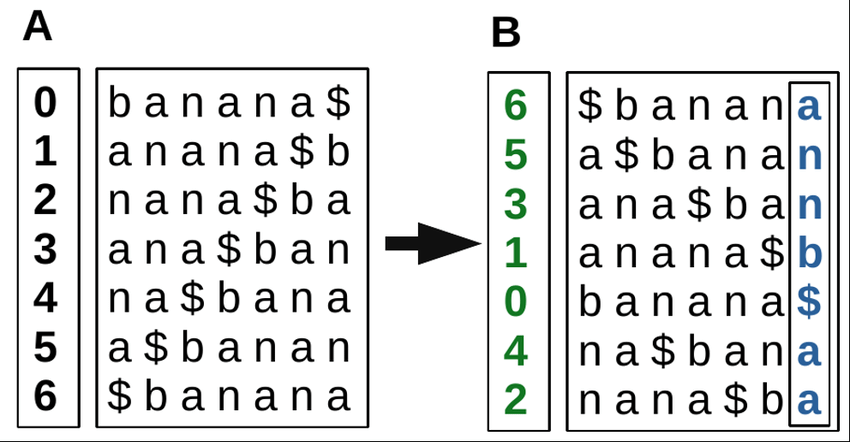
\includegraphics[width=0.5\linewidth]{images/rotation_matrix.png}
    \caption{}
    \label{fig:rotation_matrix}
\end{figure}
\begin{defn}
    Gli output della trasformazione sono la permutazione $\bwt(T)$, ovvero l'ultima colonna della matrice contenente le rotazioni di $T$ ordinate lessicograficamente, e un indice $I$, che specifica la posizione del simbolo \$ all'interno di $\bwt(T)$.
\end{defn}
\begin{rem}
    Si può notare che la colonna contenente gli indici $q$ delle $q$-rotazioni ordinate lessicograficamente corrisponde al suffix array.
\end{rem}
Essendo, per definizione di rotazione, l'ultimo simbolo di una riga $i$ della matrice ordinata il predecessore del primo simbolo dell'$i$-esima riga, ed essendo il primo simbolo della $i$-esima riga in posizione $SA[i]$, allora la BWT può essere facilmente ed efficientemente calcolata a partire dal suffix array. Sia $SA$ il suffix array, allora l'array contenente la BWT può essere calcolato come:
\[
    \bwt(T)[i] = \begin{cases}
        T[SA[i]-1] & SA[i] > 1 \\
        T[n] & SA[i] = 1
    \end{cases}
\]
La BWT "in chiaro" ha dimensione pari alla dimensione del testo $T$. Essa però gode di un'importante proprietà: essa memorizza molto spesso simboli uguali in posizioni consecutive, e può quindi essere facilmente compressa. Uno dei modi più utilizzare questa compressione è il \textbf{run-length encoding}: simboli consecutivi uguali non vengono memorizzati esplicitamente, ma viene memorizzato un solo simbolo e il numero di occorrenze consecutive del simbolo 
\footnote{Esempio: la stringa $\sigma \sigma \sigma \alpha \alpha \sigma$ verrà memorizzata come $\sigma : 3 \; \alpha : 2 \; \sigma : 1$.}.
La BWT compressa occupa quindi meno spazio in memoria rispetto al testo originale $T$, e si può quindi definire come una struttura dati succinta.

\subsubsection{Ricostruzione del testo: algoritmo ingenuo}
La ricostruzione del testo naive sfrutta la $\bwt(T)$ e la prima colonna della matrice delle rotazioni ordinate lessicograficamente, appositamente ricostruita ordinando tutti i simboli contenuti nella $\bwt(T)$.\\
Siano $F$ la prima colonna e $L$ la $\bwt(T)$, ovvero l'ultima colonna della matrice. Si può affermare che l'$i$-esimo elemento di $L$ è predecessore dell'$i$-esimo elemento di $F$, ovvero $L[i] \, F[i]$ è una stringa che compare sicuramente nel testo originale.

Concatenando $L$ e $F$ si ottiene una matrice $n \times 2$. Le righe di questa matrice possono essere ordinate lessicograficamente, e la prima riga conterrà sicuramente il prefisso di lunghezza $2$ del testo originale.
Si consideri la concatenazione seguita dall'ordinamento lessicografico delle righe come un'iterazione, è possibile definire le iterazioni seguenti come la concatenazione di $L$ e del risultato della precedente iterazione, seguita dall'ordinamento lessicografico delle righe della matrice ottenuta.\\
Alla fine della $k$-esima iterazione, la matrice conterrà nella prima riga la stringa:
\[
    \$ \, P_T[1:k]
\]
dove $P_T[1:k]$ è il prefisso di lunghezza $k$ del testo. Di conseguenza, dopo $n-1$ iterazioni, la prima riga sarà della forma:
\[
    \$ \, P_T[1:n-1]
\]
Alla $(n-1)$-esima iterazione, quindi, il testo sarà completamente ricostruito: basterà infatti spostare il simbolo \$ alla fine della stringa, ottenendo quindi il testo originale:
\[
    P_T[1:n-1] \, \$
\]

Il numero di iterazioni sono $O(n)$, e a ogni iterazione le righe della tabella devono essere ordinate lessicograficamente con un algoritmo di sorting. Ma l'algoritmo di sorting effettua $O(n \log_2n)$ confronti tra due stringhe, e ogni confronto tra due stringhe chiede $O(n)$ confronti tra simboli. Di conseguenza, la complessità dell'algoritmo di ricostruzione naive è:
\[
    O(n^3\log_2n)
\]
Dovendo costruire una matrice $n \times n$, la memoria richiesta per la ricostruzione è pari a $O(n^2)$.

\subsection*{FM-index}
L'algoritmo ingenuo di ricostruzione del testo originale a partire da $\bwt(T)$, visto nella precedente sezione, è poco efficiente sia dal punto di vista della complessità temporale che da quello della complessità spaziale.
Si può però modificare leggermente la struttura dati di indicizzazione in modo da velocizzare i tempi di esecuzione e ridurre la quantità di memoria usata, mantenendola lineare in $n$.\\
Questa struttura dati prende il nome di FM-index (METTERE CITAZIONE), e viene considerata un \textbf{compressed self-index}, in quanto permette sia di comprimere il testo originale che di indicizzare il testo, in modo da velocizzare la ricerca di pattern.

L'FM-index altro non è che la trasformata $\bwt(T)$, a cui però vengono affiancate due nuove funzioni: $\tn{C}$ e $\occ$.
Nella prossima sottosezione verrà spiegato cosa calcolano queste funzioni e perchè sono utili nella ricostruzione del testo originale.

\subsubsection{Preprocessing del testo: costruzione delle funzioni ausiliarie}
Per capire cosa calcolane le funzioni ausiliarie e perchè lo fanno è necessario prima enunciare due proprietà che valgono per la BWT.\\
\begin{property}
    $\bwt(T)[i]$ è predecessore di $T[A[i]]$. Di conseguenza, nel testo compare sicuramente la stringa:
    \[
        \bwt(T)[i] \; T[A[i]]
    \]
\end{property}
\begin{property}
    Sia $\sigma$ un simbolo che compare nel testo. L'$i$-esima occorrenza di $\sigma$ nella BWT è esattamente l'$i$-esima occorrenza di $\sigma$ nella prima colonna della tabella delle rotazioni ordinate lessicograficamente.
    Non solo sono quindi lo stesso simbolo, ma rappresentano la stessa posizione nella tabella.
\end{property}
Sia quindi $i$ la posizione del simbolo $\sigma$ nella $\bwt(T)$, allora è possibile definire una funzione che restituisce la rispettiva posizione nella prima colonna di quell'esatto simbolo $\sigma$. Questa funzione prende il nome di \textbf{last-first mapping}.
\[
    \lf: \cbra{1, \ldots, n} \rightarrow \cbra{1, \ldots, n} \quad \lf \bra{i} = \tn{C}(\sigma) + \occ \bra{i, \sigma}
\]

$\tn{C}$ e $\occ$ sono le due funzioni ausiliarie che si affiancano alla $\bwt(T)$.\\
$\tn{C}(\sigma)$ restituisce il numero di simboli nel testo $T$ che sono strettamente minori di $\sigma$, compreso \$.\\
$\occ (i, \sigma)$ restituisce, invece, il numero di occorrenze del simbolo $\sigma$ nell'intervallo $\sbra{1, i}$ della $\bwt(T)$.
\[
\tn{C}: \Sigma \rightarrow \{ 0, \ldots, n-1 \} \quad \occ: \{ 1, \ldots, n \} \times \Sigma \rightarrow \{ 0, \ldots, n \}.
\]

\subsubsection{Ricostruzione del testo}
Ricostruire il testo è possibile grazie alla BWT, alle funzioni $\tn{C}$ e $\occ$ e alle proprietà di cui gode la BWT.
Si comincia dall'ultimo simbolo del testo, ovvero \$, che si trova nella prima posizione della colonna $F$. 
Per la prima proprietà, il simbolo precedente a \$ è $L[1]$.
A sua volta $L[1]$, per la seconda proprietà, è l'esatto simbolo che si trova alla posizione $j = \lf(L[1])$ della colonna $F$. Di conseguenza, il simbolo precedente a $L[1]$ è $L[\lf(L[1])]$.
Lo stesso ragionamento può essere applicato iterativamente fino ad aver ricostruito l'intero testo.\\
L'ultima iterazione viene segnalata da $\lf(k) = 1$: se si ottiene questo valore, allora il testo è stato completamente ricostruito.